\documentclass[a4paper,UKenglish]{lipics-v2021}
\usepackage[utf8]{inputenc}%tildes
\usepackage{anysize}%cambiar margenes
\marginsize{2.25cm}{2.25cm}{1.1cm}{2.8cm}%izq,der,sup,inf
\usepackage{textcomp,gensymb}%warning Not defining(\perthousnad, \micro)
\DeclareUnicodeCharacter{0301}{\'{e}}%resolucion warning
\usepackage{amsmath, amssymb, amsthm}%Matemática avanzada
\usepackage{amsfonts, mathtools}%ampliación matemática
\usepackage{dsfont, tipa, upgreek}%math
\DeclarePairedDelimiter\norm{\lVert}{\rVert} %define norma
\usepackage{graphicx, float}%figuras y especificación H
\usepackage{setspace}%cambiar espaciado entre lineas
\setlength{\parindent}{8pt} %cambia sangría
\usepackage{enumerate}%enumerados
\usepackage{comment}
\usepackage{csquotes}
\usepackage{multicol} %varias columnas
\usepackage{biblatex}%bibliografía
\addbibresource{references.bib}%importa references

%!TEX root = ../main/main.tex

%%%%%%%%%%%%%%%%%%%%%%%%%%%%%%%%
%			PACKAGES
%%%%%%%%%%%%%%%%%%%%%%%%%%%%%%%%

\usepackage[utf8]{inputenc}
%\usepackage[english]{babel}
\usepackage{xspace}
\usepackage{algorithm}
\usepackage[noend]{algpseudocode}
\usepackage{amsmath}
\usepackage{amsthm}
\usepackage{amsfonts}
\usepackage{MnSymbol}
\usepackage{mathtools}
\usepackage{textcomp}
\usepackage{stmaryrd}
\usepackage{varwidth}
\usepackage{graphicx}
\usepackage{mathrsfs} 

\usepackage{tikz}
\usetikzlibrary{automata, graphs,positioning,chains,arrows,snakes,decorations.pathmorphing}

%%%%%%%%%%%%%%%%%%%%%%%%%%%%%%%%
%			COMMENTS
%%%%%%%%%%%%%%%%%%%%%%%%%%%%%%%%

\usepackage{todonotes}
\newcommand{\martin}[1]{\todo[inline, color=green!20]{{\bf Martin:} #1}}
\newcommand{\cristian}[1]{\todo[inline, color=red!20]{{\bf Cristian:} #1}}

%IF YOU WANT TO REMOVE COMMENTS, UNCOMMENT THE NEXT LINES
%\renewcommand{\martin}[1]{}
%\renewcommand{\cristian}[1]{}


%%%%%%%%%%%%%%%%%%%%%%%%%%%%%%%%
%			SETS
%%%%%%%%%%%%%%%%%%%%%%%%%%%%%%%%

\newcommand{\cA}{\mathcal{A}}
\newcommand{\cL}{\mathcal{L}}
\newcommand{\cO}{\mathcal{O}}
\newcommand{\cD}{\mathcal{D}}

\newcommand{\bbN}{\mathbb{N}}
\newcommand{\bbR}{\mathbb{R}}
\newcommand{\bbZ}{\mathbb{Z}}


%%%%%%%%%%%%%%%%%%%%%%%%%%%%%%%%
%			ENVIROMENTS
%%%%%%%%%%%%%%%%%%%%%%%%%%%%%%%%

\renewcommand{\paragraph}[1]{\smallskip
	\noindent\textbf{#1}.}

%%%%%%%%%%%%%%%%%%%%%%%%%%%%%%%%
%			ALGORITHMS
%%%%%%%%%%%%%%%%%%%%%%%%%%%%%%%%

\renewcommand{\operatorname}[1]{\mathsf{#1}}

\algrenewcommand\algorithmicindent{1.3em}%
\algnewcommand\algorithmicforeach{\textbf{for each}}
\algdef{S}[FOR]{ForEach}[1]{\algorithmicforeach\ #1\ \algorithmicdo}




%!TEX root = ../main/main.tex

\bibliographystyle{plainurl}% the mandatory bibstyle

\title{Horton–Strahler number and centrality measures} 
\titlerunning{Horton–Strahler number and centrality measures} 


\author{Carlos Olguin}{Pontificia Universidad Católica de Chile}{carlosfelipeolguin@uc.cl}{}{}
%\author{Cristian Riveros}{Pontificia Universidad Católica de Chile}{cristian.riveros@uc.cl}{}{}

\authorrunning{Carlos Olguin}
\Copyright{Carlos Olguin}

\ccsdesc[500]{Theory of computation~Database theory}
%\ccsdesc[100]{General and reference~General literature}
%\ccsdesc[100]{General and reference}%TODO mandatory: Please choose ACM 2012 classifications from https://dl.acm.org/ccs/ccs_flat.cfm 

\keywords{Horton-Strahler number, centrality measures}

%\relatedversion{}
%\relatedversiondetails{Extended Version}{https://arxiv.org/abs/2010.06037}


%\nolinenumbers %uncomment to disable line numbering

\hideLIPIcs  %uncomment to remove references to LIPIcs series (logo, DOI, ...), e.g. when preparing a pre-final version to be uploaded to arXiv or another public repository

%\funding{This work was funded by ANID - Millennium Science Initiative Program - Code {\tt ICN17\_002.}}

%Editor-only macros:: begin (do not touch as author)%%%%%%%%%%%%%%%%%%%%%%%%%%%%%%%%%%
%\EventEditors{Dan Olteanu and Nils Vortmeier}
%\EventNoEds{2}
%\EventLongTitle{25th International Conference on Database Theory (ICDT 2022)}
%\EventShortTitle{ICDT 2022}
%\EventAcronym{ICDT}
%\EventYear{2022}
%\EventDate{March 29--April 1, 2022}
%\EventLocation{Edinburgh, UK}
%\EventLogo{}
%\SeriesVolume{220}
%\ArticleNo{8}
%%%%%%%%%%%%%%%%%%%%%%%%%%%%%%%%%%%%%%%%%%%%%%%%%%%%%%

\begin{document}
	
	\maketitle
	
	%!TEX root = ../main/main.tex

\begin{abstract}

Centrality measures are widely used to assign importance to graph-structured data. This approach to graph analysis has provided various interpretations for different graphs, allowing us to formalize concepts such as graph importance using these measures. In a previous paper, we presented the formalization of these concepts, utilizing potential functions to capture the rooting property of different centralities. In this paper, we analyse the concept of the Strahler number as a centrality and examine different properties and beyond.

\end{abstract}
	
	\section{Introduction}\label{sec:introduction}
	
	%!TEX root = ../main/main.tex
In this paper, we will address different topics such as graphs, centralities in graphs, and the central concept in this paper, the Strahler Number. With this concept of the Strahler number, we will approach using different tools previously defined in the previous paper in order to find a relation between the Strahler number and centrality in a graph. First, we will define important concepts such as centrality, a tree, etc. Next, we will provide a definition of the Strahler number, and finally, we will explore (if any) the relationships between the tools we defined and the Strahler number, as well as some projections and remaining work to be done.
	
	\section{Preliminaries}\label{sec:preliminaries}
	
	%!TEX root = ../main/main.tex

\paragraph{Graphs} A graph is a pair $G = (V, E)$ where $V$ is a finite set and $E \subseteq V\times V$ is a finite relation. Each par of vertex let be $(v_{1},v_{2})$ , $v_{1},v_{2} \in V$ this set of vertex its called edges and can be directed or not, so the edges $\in E$. A path in a graph is a sequence of non-repeated nodes connected through edges present in a graph, if there exist a path between two vertex, this vertex are called connected. An example, let be $x,y \in V$ a path can be expressed so $\{x,x_{1},x_{2},\cdots,y_{1},y_{2},\cdots,y_{n} \}$ with $x,x_{i},y_{i},y \in V$

\paragraph{Trees} A tree is an undirected graph in which any two vertices are connected by only and only one path. A rooted tree is refereed as a tree with a vertex who serves as the "root" of the tree, being a references to the others  vertices in the tree.  

\paragraph{Aplicacions}   




	
	\section{Main results}\label{sec:results}
	
	%!TEX root = ../main/main.tex

We can observe that the Strahler number is similar to a centrality measure, in a sense which, is a function who takes a node an assigns a score (with certain conditions). That is why the co-relation between Strahler number is visible. We can define the centrality measure using Strahler number in a sense that a higher Strahler number means higher centrality. It is important to remember that a potential function tell us if a centrality measure is able to root trees. In other words, if a centrality measure admits a potential function, it will roots trees if, and only if, the potential function is symmetric (not necessarily works backwards). It is valid to ask if this centrality roots trees, we can approach this by defining a a potential function. Specifically, taking the concept of Strahler number we define the following a potential function for a vertex $v$ of a tree $T$:
    \begin{equation*}
        f_{S_{N}} (v,T) = \left\{ \begin{array}{llc}
             1 &   \text{if $v$ is a leaf of $T$ (i.e., $v$ does not have children)}  & \smallskip \\ 
              i & \text{if $v$ has one child $u$ with $f_{S_{N}}(u, T) = i$, and} \\
              	& \text{all other children have  $f_{S_{N}} < i$} \smallskip \\
              i + 1 &  \text{if $v$ has two or more children $u$ with $f_{S_{N}}(u, T) = i$} \\
              & \text{and no other children with $f_{S_{N}} > i$.} \\
             \end{array}
   \right.
    \end{equation*}
    
We can see that this potential function makes sense because the potential of a node it depends of their children (by definition of Strahler number).

We can see now if this function is symmetric knowing that the concept of the Strahler number, is to represent a directed graph and measure the centrality to different contexts. We can make a counter-example for this and observe that if we consider the graph:
\begin{center}
        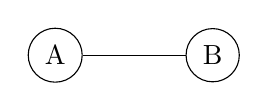
\begin{tikzpicture}
        \node[circle, draw] (A) at (0,0) {A};
        \node[circle, draw] (B) at (2,0) {B};

        \draw (A) -- (B);
    \end{tikzpicture}
\end{center}
\cristian{Falta arreglar este ejemplo. No esta según lo que dices abajo.}
In this example we can observe that the centrality goes to the center in the way of $A$ to $B$ and $D$ to $C$, such that, $f(A,T_{A,B}) =  f(B,T) = 0$ in such way that this is not symmetrical and in this sense does not root trees.

Knowing that this admits a potential function $f$ and $f$ is not symmetrical, by Theorem 11 in~\cite{RiverosSS23} it will not root trees. In other words, we cannot find the root of tree in all cases with this centrality. 

If this centrality does not roots trees we can explore other things like if this potential function in a monoids version, such this cannot happen because we can observe that, this potential function implies a monoid that is not associative (which is not a monoid by definition), such leaf function can be drafted like:
\begin{equation}
    \max\{ x,y \}= \left\{ \begin{array}{lcc}
              \max\{x,y \} &   if  & x \neq y \\
             \\ \max\{ x,y \} + 1 & if  & x = y 
             \end{array}
   \right.
\end{equation}
This function can represent correctly the centrality of a single vertex , but, it can not represent a potential function (recursively) because is not associative (and thus is not a monoid). For example,
\begin{equation}
    \max\{ 1,\max\{ 1,2 \} \} = 2 \\
    \vspace{0.5cm}
    \max\{ \max\{ 1,1 \},2 \}  = 3 \\
    \vspace{0.5cm}
    \rightarrow 2 \neq 3
\end{equation}
If this centrality can not root trees this means, we can not find a root for a tree $T$, which can be a problem in different applications.



	
	\section{Conclusions}\label{sec:conclusions}
	
	%!TEX root = main.tex

Lorem ipsum dolor sit amet, consectetur adipiscing elit, sed do eiusmod tempor incididunt ut labore et dolore magna aliqua. Ut enim ad minim veniam, quis nostrud exercitation ullamco laboris nisi ut aliquip ex ea commodo consequat. Duis aute irure dolor in reprehenderit in voluptate velit esse cillum dolore eu fugiat nulla pariatur. Excepteur sint occaecat cupidatat non proident, sunt in culpa qui officia deserunt mollit anim id est laborum.
	
	\newpage
	\bibliographystyle{abbrv}
	\bibliography{../extras/biblio}
	
	\newpage
	\appendix
	
	\section{Proofs from Section~\ref{sec:preliminaries}}
	
	%!TEX root = ../main/main.tex

Lorem ipsum dolor sit amet, consectetur adipiscing elit, sed do eiusmod tempor incididunt ut labore et dolore magna aliqua. Ut enim ad minim veniam, quis nostrud exercitation ullamco laboris nisi ut aliquip ex ea commodo consequat. Duis aute irure dolor in reprehenderit in voluptate velit esse cillum dolore eu fugiat nulla pariatur. Excepteur sint occaecat cupidatat non proident, sunt in culpa qui officia deserunt mollit anim id est laborum.
	
	\section{Proofs of Section~\ref{sec:results}}
	
	%!TEX root = ../main/main.tex

\subsection{Proof of Lemma~\ref{lemma:mylemma}}

Lorem ipsum dolor sit amet, consectetur adipiscing elit, sed do eiusmod tempor incididunt ut labore et dolore magna aliqua. Ut enim ad minim veniam, quis nostrud exercitation ullamco laboris nisi ut aliquip ex ea commodo consequat. Duis aute irure dolor in reprehenderit in voluptate velit esse cillum dolore eu fugiat nulla pariatur. Excepteur sint occaecat cupidatat non proident, sunt in culpa qui officia deserunt mollit anim id est laborum.

\begin{figure}[t]
	\centering
	%!TEX root = main.tex

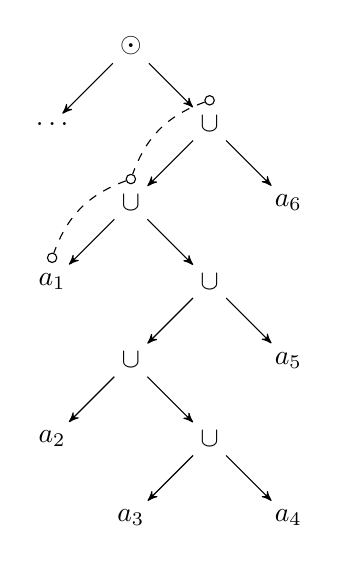
\begin{tikzpicture}[->,>=stealth',roundnode/.style={circle,draw,inner sep=1.2pt},squarednode/.style={rectangle,inner sep=3pt}]
	
	\node [squarednode] (0) at (1, 0) {$a_3$};
%	\node [roundnode] (0b) at (1, 0.3) {};
	\node [squarednode] (1) at (3, 0) {$a_4$};
%	\node [roundnode] (1b) at (3, 0.3) {};
	\node [squarednode] (2) at (2, 1) {$\cup$};
%	\node [roundnode] (2b) at (2, 1.3) {};
	\node [squarednode] (3) at (0, 1) {$a_2$};
%	\node [roundnode] (3b) at (0, 1.3) {};
	\node [squarednode] (4) at (1, 2) {$\cup$};
%	\node [roundnode] (4b) at (1, 2.3) {};
	\node [squarednode] (5) at (3, 2) {$a_5$};
%	\node [roundnode] (5b) at (3, 2.3) {};
	\node [squarednode] (6) at (2, 3) {$\cup$};
%	\node [roundnode] (6b) at (2, 3.3) {};
	\node [squarednode] (7) at (0, 3) {$a_1$};
	\node [roundnode] (7b) at (0, 3.3) {};
	\node [squarednode] (8) at (1, 4) {$\cup$};
	\node [roundnode] (8b) at (1, 4.3) {};
	\node [squarednode] (9) at (3, 4) {$a_6$};
%	\node [roundnode] (9b) at (3, 4.3) {};
	\node [squarednode] (10) at (2, 5) {$\cup$};
	\node [roundnode] (10b) at (2, 5.3) {};
	\node [squarednode] (11) at (0, 5) {$\ldots$};
	\node [squarednode] (12) at (1, 6) {$\odot$};
%	\node [roundnode] (12b) at (1, 6.3) {};
	
	\draw (2) to (0);
	\draw (2) to (1);
	\draw (4) to (2);
	\draw (4) to (3);
	\draw (6) to (4);
	\draw (6) to (5);
	\draw (8) to (6);
	\draw (8) to (7);
	\draw (10) to (8);
	\draw (10) to (9);
	\draw (12) to (10);
	\draw (12) to (11);
	
%	\draw[dashed, -, out=200, in=70] (12b) to (10b);
	\draw[dashed, -, out=200, in=70] (10b) to (8b);
	\draw[dashed, -, out=200, in=70] (8b) to (7b);
%	\draw[dashed, -, out=200, in=110] (10b) to (6b);
%	\draw[dashed, -, out=200, in=70] (6b) to (4b);
%	\draw[dashed, -, out=200, in=70] (4b) to (3b);
%	\draw[dashed, -, out=200, in=110] (6b) to (2b);
%	\draw[dashed, -, out=200, in=70] (2b) to (0b);
%	\draw[dashed, -, out=200, in=110] (6b) to (1b);
%	\draw[dashed, -, out=200, in=110] (10b) to (5b);
%	\draw[dashed, -, out=200, in=110] (12b) to (9b);

\end{tikzpicture}
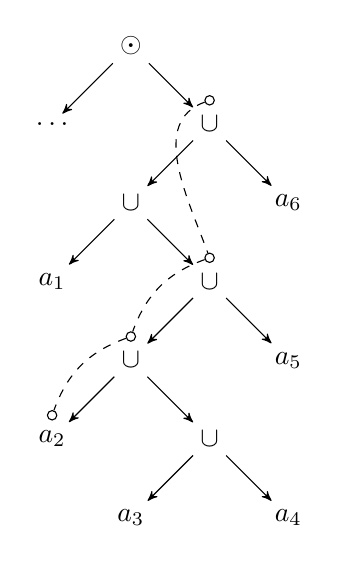
\begin{tikzpicture}[->,>=stealth',roundnode/.style={circle,draw,inner sep=1.2pt},squarednode/.style={rectangle,inner sep=3pt}]
	
	\node [squarednode] (0) at (1, 0) {$a_3$};
%	\node [roundnode] (0b) at (1, 0.3) {};
	\node [squarednode] (1) at (3, 0) {$a_4$};
%	\node [roundnode] (1b) at (3, 0.3) {};
	\node [squarednode] (2) at (2, 1) {$\cup$};
%	\node [roundnode] (2b) at (2, 1.3) {};
	\node [squarednode] (3) at (0, 1) {$a_2$};
	\node [roundnode] (3b) at (0, 1.3) {};
	\node [squarednode] (4) at (1, 2) {$\cup$};
	\node [roundnode] (4b) at (1, 2.3) {};
	\node [squarednode] (5) at (3, 2) {$a_5$};
%	\node [roundnode] (5b) at (3, 2.3) {};
	\node [squarednode] (6) at (2, 3) {$\cup$};
	\node [roundnode] (6b) at (2, 3.3) {};
	\node [squarednode] (7) at (0, 3) {$a_1$};
%	\node [roundnode] (7b) at (0, 3.3) {};
	\node [squarednode] (8) at (1, 4) {$\cup$};
%	\node [roundnode] (8b) at (1, 4.3) {};
	\node [squarednode] (9) at (3, 4) {$a_6$};
%	\node [roundnode] (9b) at (3, 4.3) {};
	\node [squarednode] (10) at (2, 5) {$\cup$};
	\node [roundnode] (10b) at (2, 5.3) {};
	\node [squarednode] (11) at (0, 5) {$\ldots$};
	\node [squarednode] (12) at (1, 6) {$\odot$};
	%	\node [roundnode] (12b) at (1, 6.3) {};
	
	\draw (2) to (0);
	\draw (2) to (1);
	\draw (4) to (2);
	\draw (4) to (3);
	\draw (6) to (4);
	\draw (6) to (5);
	\draw (8) to (6);
	\draw (8) to (7);
	\draw (10) to (8);
	\draw (10) to (9);
	\draw (12) to (10);
	\draw (12) to (11);
	
%	\draw[dashed, -, out=200, in=70] (12b) to (10b);
%	\draw[dashed, -, out=200, in=70] (10b) to (8b);
%	\draw[dashed, -, out=200, in=70] (8b) to (7b);
	\draw[dashed, -, out=200, in=110] (10b) to (6b);
	\draw[dashed, -, out=200, in=70] (6b) to (4b);
	\draw[dashed, -, out=200, in=70] (4b) to (3b);
%	\draw[dashed, -, out=200, in=110] (6b) to (2b);
%	\draw[dashed, -, out=200, in=70] (2b) to (0b);
%	\draw[dashed, -, out=200, in=110] (6b) to (1b);
%	\draw[dashed, -, out=200, in=110] (10b) to (5b);
%	\draw[dashed, -, out=200, in=110] (12b) to (9b);
\end{tikzpicture}
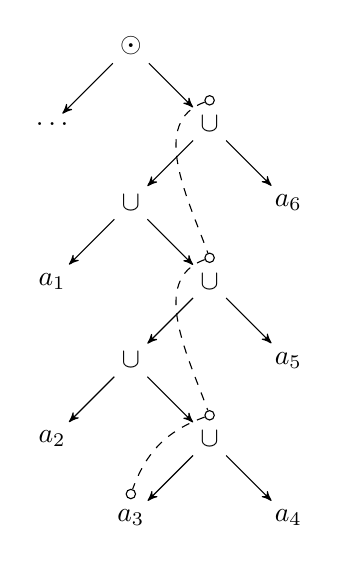
\begin{tikzpicture}[->,>=stealth',roundnode/.style={circle,draw,inner sep=1.2pt},squarednode/.style={rectangle,inner sep=3pt}]
	
	\node [squarednode] (0) at (1, 0) {$a_3$};
	\node [roundnode] (0b) at (1, 0.3) {};
	\node [squarednode] (1) at (3, 0) {$a_4$};
%	\node [roundnode] (1b) at (3, 0.3) {};
	\node [squarednode] (2) at (2, 1) {$\cup$};
	\node [roundnode] (2b) at (2, 1.3) {};
	\node [squarednode] (3) at (0, 1) {$a_2$};
%	\node [roundnode] (3b) at (0, 1.3) {};
	\node [squarednode] (4) at (1, 2) {$\cup$};
%	\node [roundnode] (4b) at (1, 2.3) {};
	\node [squarednode] (5) at (3, 2) {$a_5$};
%	\node [roundnode] (5b) at (3, 2.3) {};
	\node [squarednode] (6) at (2, 3) {$\cup$};
	\node [roundnode] (6b) at (2, 3.3) {};
	\node [squarednode] (7) at (0, 3) {$a_1$};
%	\node [roundnode] (7b) at (0, 3.3) {};
	\node [squarednode] (8) at (1, 4) {$\cup$};
%	\node [roundnode] (8b) at (1, 4.3) {};
	\node [squarednode] (9) at (3, 4) {$a_6$};
%	\node [roundnode] (9b) at (3, 4.3) {};
	\node [squarednode] (10) at (2, 5) {$\cup$};
	\node [roundnode] (10b) at (2, 5.3) {};
	\node [squarednode] (11) at (0, 5) {$\ldots$};
	\node [squarednode] (12) at (1, 6) {$\odot$};
	%	\node [roundnode] (12b) at (1, 6.3) {};
	
	\draw (2) to (0);
	\draw (2) to (1);
	\draw (4) to (2);
	\draw (4) to (3);
	\draw (6) to (4);
	\draw (6) to (5);
	\draw (8) to (6);
	\draw (8) to (7);
	\draw (10) to (8);
	\draw (10) to (9);
	\draw (12) to (10);
	\draw (12) to (11);
	
%	\draw[dashed, -, out=200, in=70] (12b) to (10b);
%	\draw[dashed, -, out=200, in=70] (10b) to (8b);
%	\draw[dashed, -, out=200, in=70] (8b) to (7b);
	\draw[dashed, -, out=200, in=110] (10b) to (6b);
%	\draw[dashed, -, out=200, in=70] (6b) to (4b);
%	\draw[dashed, -, out=200, in=70] (4b) to (3b);
	\draw[dashed, -, out=200, in=110] (6b) to (2b);
	\draw[dashed, -, out=200, in=70] (2b) to (0b);
%	\draw[dashed, -, out=200, in=110] (6b) to (1b);
%	\draw[dashed, -, out=200, in=110] (10b) to (5b);
%	\draw[dashed, -, out=200, in=110] (12b) to (9b);
\end{tikzpicture}

\vspace{1em}

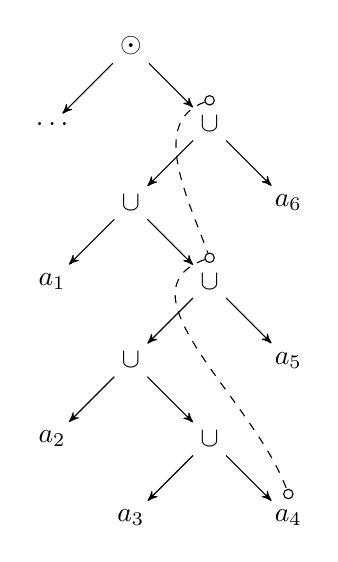
\begin{tikzpicture}[->,>=stealth',roundnode/.style={circle,draw,inner sep=1.2pt},squarednode/.style={rectangle,inner sep=3pt}]
	
	\node [squarednode] (0) at (1, 0) {$a_3$};
%	\node [roundnode] (0b) at (1, 0.3) {};
	\node [squarednode] (1) at (3, 0) {$a_4$};
	\node [roundnode] (1b) at (3, 0.3) {};
	\node [squarednode] (2) at (2, 1) {$\cup$};
%	\node [roundnode] (2b) at (2, 1.3) {};
	\node [squarednode] (3) at (0, 1) {$a_2$};
%	\node [roundnode] (3b) at (0, 1.3) {};
	\node [squarednode] (4) at (1, 2) {$\cup$};
%	\node [roundnode] (4b) at (1, 2.3) {};
	\node [squarednode] (5) at (3, 2) {$a_5$};
%	\node [roundnode] (5b) at (3, 2.3) {};
	\node [squarednode] (6) at (2, 3) {$\cup$};
	\node [roundnode] (6b) at (2, 3.3) {};
	\node [squarednode] (7) at (0, 3) {$a_1$};
%	\node [roundnode] (7b) at (0, 3.3) {};
	\node [squarednode] (8) at (1, 4) {$\cup$};
%	\node [roundnode] (8b) at (1, 4.3) {};
	\node [squarednode] (9) at (3, 4) {$a_6$};
%	\node [roundnode] (9b) at (3, 4.3) {};
	\node [squarednode] (10) at (2, 5) {$\cup$};
	\node [roundnode] (10b) at (2, 5.3) {};
	\node [squarednode] (11) at (0, 5) {$\ldots$};
	\node [squarednode] (12) at (1, 6) {$\odot$};
	%	\node [roundnode] (12b) at (1, 6.3) {};
	
	\draw (2) to (0);
	\draw (2) to (1);
	\draw (4) to (2);
	\draw (4) to (3);
	\draw (6) to (4);
	\draw (6) to (5);
	\draw (8) to (6);
	\draw (8) to (7);
	\draw (10) to (8);
	\draw (10) to (9);
	\draw (12) to (10);
	\draw (12) to (11);
	
%	\draw[dashed, -, out=200, in=70] (12b) to (10b);
%	\draw[dashed, -, out=200, in=70] (10b) to (8b);
%	\draw[dashed, -, out=200, in=70] (8b) to (7b);
	\draw[dashed, -, out=200, in=110] (10b) to (6b);
%	\draw[dashed, -, out=200, in=70] (6b) to (4b);
%	\draw[dashed, -, out=200, in=70] (4b) to (3b);
%	\draw[dashed, -, out=200, in=110] (6b) to (2b);
%	\draw[dashed, -, out=200, in=70] (2b) to (0b);
	\draw[dashed, -, out=200, in=110] (6b) to (1b);
%	\draw[dashed, -, out=200, in=110] (10b) to (5b);
%	\draw[dashed, -, out=200, in=110] (12b) to (9b);
\end{tikzpicture}
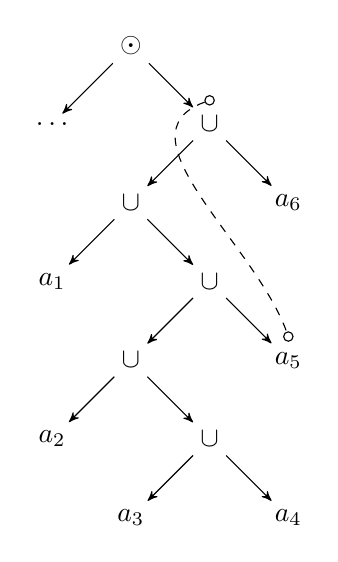
\begin{tikzpicture}[->,>=stealth',roundnode/.style={circle,draw,inner sep=1.2pt},squarednode/.style={rectangle,inner sep=3pt}]
	
	\node [squarednode] (0) at (1, 0) {$a_3$};
%	\node [roundnode] (0b) at (1, 0.3) {};
	\node [squarednode] (1) at (3, 0) {$a_4$};
%	\node [roundnode] (1b) at (3, 0.3) {};
	\node [squarednode] (2) at (2, 1) {$\cup$};
%	\node [roundnode] (2b) at (2, 1.3) {};
	\node [squarednode] (3) at (0, 1) {$a_2$};
%	\node [roundnode] (3b) at (0, 1.3) {};
	\node [squarednode] (4) at (1, 2) {$\cup$};
%	\node [roundnode] (4b) at (1, 2.3) {};
	\node [squarednode] (5) at (3, 2) {$a_5$};
	\node [roundnode] (5b) at (3, 2.3) {};
	\node [squarednode] (6) at (2, 3) {$\cup$};
%	\node [roundnode] (6b) at (2, 3.3) {};
	\node [squarednode] (7) at (0, 3) {$a_1$};
%	\node [roundnode] (7b) at (0, 3.3) {};
	\node [squarednode] (8) at (1, 4) {$\cup$};
%	\node [roundnode] (8b) at (1, 4.3) {};
	\node [squarednode] (9) at (3, 4) {$a_6$};
%	\node [roundnode] (9b) at (3, 4.3) {};
	\node [squarednode] (10) at (2, 5) {$\cup$};
	\node [roundnode] (10b) at (2, 5.3) {};
	\node [squarednode] (11) at (0, 5) {$\ldots$};
	\node [squarednode] (12) at (1, 6) {$\odot$};
	%	\node [roundnode] (12b) at (1, 6.3) {};
	
	\draw (2) to (0);
	\draw (2) to (1);
	\draw (4) to (2);
	\draw (4) to (3);
	\draw (6) to (4);
	\draw (6) to (5);
	\draw (8) to (6);
	\draw (8) to (7);
	\draw (10) to (8);
	\draw (10) to (9);
	\draw (12) to (10);
	\draw (12) to (11);
	
%	\draw[dashed, -, out=200, in=70] (12b) to (10b);
%	\draw[dashed, -, out=200, in=70] (10b) to (8b);
%	\draw[dashed, -, out=200, in=70] (8b) to (7b);
%	\draw[dashed, -, out=200, in=110] (10b) to (6b);
%	\draw[dashed, -, out=200, in=70] (6b) to (4b);
%	\draw[dashed, -, out=200, in=70] (4b) to (3b);
%	\draw[dashed, -, out=200, in=110] (6b) to (2b);
%	\draw[dashed, -, out=200, in=70] (2b) to (0b);
%	\draw[dashed, -, out=200, in=110] (6b) to (1b);
	\draw[dashed, -, out=200, in=110] (10b) to (5b);
%	\draw[dashed, -, out=200, in=110] (12b) to (9b);
\end{tikzpicture}
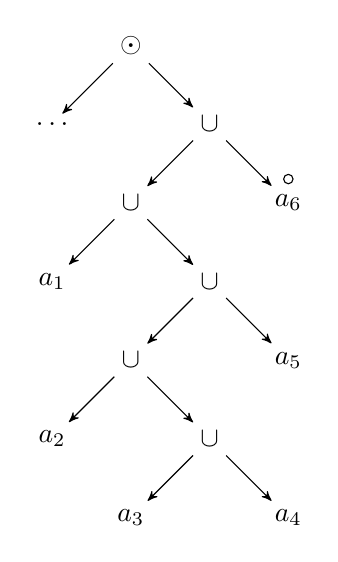
\begin{tikzpicture}[->,>=stealth',roundnode/.style={circle,draw,inner sep=1.2pt},squarednode/.style={rectangle,inner sep=3pt}]

\node [squarednode] (0) at (1, 0) {$a_3$};
%\node [roundnode] (0b) at (1, 0.3) {};
\node [squarednode] (1) at (3, 0) {$a_4$};
%\node [roundnode] (1b) at (3, 0.3) {};
\node [squarednode] (2) at (2, 1) {$\cup$};
%\node [roundnode] (2b) at (2, 1.3) {};
\node [squarednode] (3) at (0, 1) {$a_2$};
%\node [roundnode] (3b) at (0, 1.3) {};
\node [squarednode] (4) at (1, 2) {$\cup$};
%\node [roundnode] (4b) at (1, 2.3) {};
\node [squarednode] (5) at (3, 2) {$a_5$};
%\node [roundnode] (5b) at (3, 2.3) {};
\node [squarednode] (6) at (2, 3) {$\cup$};
%\node [roundnode] (6b) at (2, 3.3) {};
\node [squarednode] (7) at (0, 3) {$a_1$};
%\node [roundnode] (7b) at (0, 3.3) {};
\node [squarednode] (8) at (1, 4) {$\cup$};
%\node [roundnode] (8b) at (1, 4.3) {};
\node [squarednode] (9) at (3, 4) {$a_6$};
\node [roundnode] (9b) at (3, 4.3) {};
\node [squarednode] (10) at (2, 5) {$\cup$};
%\node [roundnode] (10b) at (2, 5.3) {};
\node [squarednode] (11) at (0, 5) {$\ldots$};
\node [squarednode] (12) at (1, 6) {$\odot$};
%	\node [roundnode] (12b) at (1, 6.3) {};

\draw (2) to (0);
\draw (2) to (1);
\draw (4) to (2);
\draw (4) to (3);
\draw (6) to (4);
\draw (6) to (5);
\draw (8) to (6);
\draw (8) to (7);
\draw (10) to (8);
\draw (10) to (9);
\draw (12) to (10);
\draw (12) to (11);

%\draw[dashed, -, out=200, in=70] (12b) to (10b);
%\draw[dashed, -, out=200, in=70] (10b) to (8b);
%\draw[dashed, -, out=200, in=70] (8b) to (7b);
%\draw[dashed, -, out=200, in=110] (10b) to (6b);
%\draw[dashed, -, out=200, in=70] (6b) to (4b);
%\draw[dashed, -, out=200, in=70] (4b) to (3b);
%\draw[dashed, -, out=200, in=110] (6b) to (2b);
%\draw[dashed, -, out=200, in=70] (2b) to (0b);
%\draw[dashed, -, out=200, in=110] (6b) to (1b);
%\draw[dashed, -, out=200, in=110] (10b) to (5b);
%\draw[dashed, -, out=200, in=110] (12b) to (9b);
\end{tikzpicture}
	\caption{An example iteration of ${\tt trav}$ and ${\tt move}$. The sequences of nodes joined by dashed lines represent a stack $\mathsf{St}$, where the first one was obtained after calling ${\tt trav}$ over the topmost union node, and the following five are obtained by repeated applications of ${\tt move}(\mathsf{St})$.}
	\label{fig-enum-stacks}
\end{figure}

Lorem ipsum dolor sit amet, consectetur adipiscing elit, sed do eiusmod tempor incididunt ut labore et dolore magna aliqua. Ut enim ad minim veniam, quis nostrud exercitation ullamco laboris nisi ut aliquip ex ea commodo consequat. Duis aute irure dolor in reprehenderit in voluptate velit esse cillum dolore eu fugiat nulla pariatur. Excepteur sint occaecat cupidatat non proident, sunt in culpa qui officia deserunt mollit anim id est laborum.

Lorem ipsum dolor sit amet, consectetur adipiscing elit, sed do eiusmod tempor incididunt ut labore et dolore magna aliqua. Ut enim ad minim veniam, quis nostrud exercitation ullamco laboris nisi ut aliquip ex ea commodo consequat. Duis aute irure dolor in reprehenderit in voluptate velit esse cillum dolore eu fugiat nulla pariatur. Excepteur sint occaecat cupidatat non proident, sunt in culpa qui officia deserunt mollit anim id est laborum.

Lorem ipsum dolor sit amet, consectetur adipiscing elit, sed do eiusmod tempor incididunt ut labore et dolore magna aliqua. Ut enim ad minim veniam, quis nostrud exercitation ullamco laboris nisi ut aliquip ex ea commodo consequat. Duis aute irure dolor in reprehenderit in voluptate velit esse cillum dolore eu fugiat nulla pariatur. Excepteur sint occaecat cupidatat non proident, sunt in culpa qui officia deserunt mollit anim id est laborum.

Lorem ipsum dolor sit amet, consectetur adipiscing elit, sed do eiusmod tempor incididunt ut labore et dolore magna aliqua. Ut enim ad minim veniam, quis nostrud exercitation ullamco laboris nisi ut aliquip ex ea commodo consequat. Duis aute irure dolor in reprehenderit in voluptate velit esse cillum dolore eu fugiat nulla pariatur. Excepteur sint occaecat cupidatat non proident, sunt in culpa qui officia deserunt mollit anim id est laborum.

Lorem ipsum dolor sit amet, consectetur adipiscing elit, sed do eiusmod tempor incididunt ut labore et dolore magna aliqua. Ut enim ad minim veniam, quis nostrud exercitation ullamco laboris nisi ut aliquip ex ea commodo consequat. Duis aute irure dolor in reprehenderit in voluptate velit esse cillum dolore eu fugiat nulla pariatur. Excepteur sint occaecat cupidatat non proident, sunt in culpa qui officia deserunt mollit anim id est laborum.


\subsection{Proof of Theorem~\ref{theo:mytheorem}}

Lorem ipsum dolor sit amet, consectetur adipiscing elit, sed do eiusmod tempor incididunt ut labore et dolore magna aliqua. Ut enim ad minim veniam, quis nostrud exercitation ullamco laboris nisi ut aliquip ex ea commodo consequat. Duis aute irure dolor in reprehenderit in voluptate velit esse cillum dolore eu fugiat nulla pariatur. Excepteur sint occaecat cupidatat non proident, sunt in culpa qui officia deserunt mollit anim id est laborum.

%!TEX root = main.tex

\begin{figure}
	\centering
	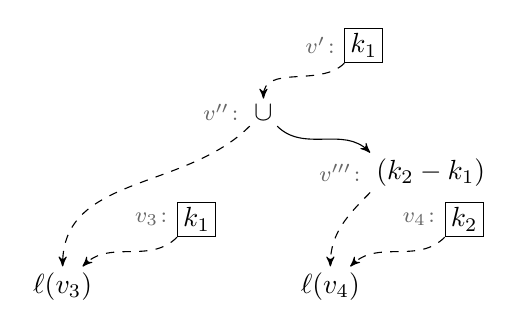
\begin{tikzpicture}[every label/.style={black!60}, ->,>=stealth',roundnode/.style={circle,inner sep=1pt},squarednode/.style={rectangle,inner sep=2pt}, scale=0.85]
		\node[squarednode] (0) at (0, 0) {$\ell(v_3)$};
		\node[squarednode, draw, label=180:\footnotesize{$v_3\!:$}] (2) at (2, 1) {$k_1$};
		\node[squarednode] (3) at (4, 0) {$\ell(v_4)$};
		\node[squarednode, draw, label=180:\footnotesize{$v_4\!:$}] (5) at (6, 1) {$k_2$};
		\node[squarednode, label=180:\footnotesize{$v'''\!:$}] (7) at (5.5, 1.7) {$(k_2-k_1)$};
		\node[squarednode, label=180:\footnotesize{$v''\!:$}] (8) at (3, 2.6) {$\cup$};
		\node[squarednode, draw, label=180:\footnotesize{$v'\!:$}] (9) at (4.5, 3.6) {$k_1$};
		\draw[dashed] (2.south west) to[out=-135,in=45] (0);
		\draw[dashed] (5.south west) to[out=-135,in=45] (3);
		\draw[dashed] (7.south west) to[out=-135,in=90] (3);
		\draw (8) to[out=-45,in=135] (7.north west);
		\draw[dashed] (8) to[out=-135,in=90] (0);
		\draw[dashed] (9.south west) to[out=-135,in=90] (8);
		
	\end{tikzpicture}
	\caption{Gadget used in Theorem~\ref{theo:mytheorem}.}
	\label{fig-theo-ds}
\end{figure}

Lorem ipsum dolor sit amet, consectetur adipiscing elit, sed do eiusmod tempor incididunt ut labore et dolore magna aliqua. Ut enim ad minim veniam, quis nostrud exercitation ullamco laboris nisi ut aliquip ex ea commodo consequat. Duis aute irure dolor in reprehenderit in voluptate velit esse cillum dolore eu fugiat nulla pariatur. Excepteur sint occaecat cupidatat non proident, sunt in culpa qui officia deserunt mollit anim id est laborum.
Lorem ipsum dolor sit amet, consectetur adipiscing elit, sed do eiusmod tempor incididunt ut labore et dolore magna aliqua. Ut enim ad minim veniam, quis nostrud exercitation ullamco laboris nisi ut aliquip ex ea commodo consequat. Duis aute irure dolor in reprehenderit in voluptate velit esse cillum dolore eu fugiat nulla pariatur. Excepteur sint occaecat cupidatat non proident, sunt in culpa qui officia deserunt mollit anim id est laborum.

Lorem ipsum dolor sit amet, consectetur adipiscing elit, sed do eiusmod tempor incididunt ut labore et dolore magna aliqua. Ut enim ad minim veniam, quis nostrud exercitation ullamco laboris nisi ut aliquip ex ea commodo consequat. Duis aute irure dolor in reprehenderit in voluptate velit esse cillum dolore eu fugiat nulla pariatur. Excepteur sint occaecat cupidatat non proident, sunt in culpa qui officia deserunt mollit anim id est laborum.

Lorem ipsum dolor sit amet, consectetur adipiscing elit, sed do eiusmod tempor incididunt ut labore et dolore magna aliqua. Ut enim ad minim veniam, quis nostrud exercitation ullamco laboris nisi ut aliquip ex ea commodo consequat. Duis aute irure dolor in reprehenderit in voluptate velit esse cillum dolore eu fugiat nulla pariatur. Excepteur sint occaecat cupidatat non proident, sunt in culpa qui officia deserunt mollit anim id est laborum.

Lorem ipsum dolor sit amet, consectetur adipiscing elit, sed do eiusmod tempor incididunt ut labore et dolore magna aliqua. Ut enim ad minim veniam, quis nostrud exercitation ullamco laboris nisi ut aliquip ex ea commodo consequat. Duis aute irure dolor in reprehenderit in voluptate velit esse cillum dolore eu fugiat nulla pariatur. Excepteur sint occaecat cupidatat non proident, sunt in culpa qui officia deserunt mollit anim id est laborum.

\subsection{Proof of Proposition~\ref{prop:myproposition}}

Lorem ipsum dolor sit amet, consectetur adipiscing elit, sed do eiusmod tempor incididunt ut labore et dolore magna aliqua. Ut enim ad minim veniam, quis nostrud exercitation ullamco laboris nisi ut aliquip ex ea commodo consequat. Duis aute irure dolor in reprehenderit in voluptate velit esse cillum dolore eu fugiat nulla pariatur. Excepteur sint occaecat cupidatat non proident, sunt in culpa qui officia deserunt mollit anim id est laborum.

\begin{claim}\label{prop:lindelayeps}
	Fix $k\in\bbN$. Let $\mathcal{C}_k$ be the class of all  duplicate-free and $k$-bounded $D$ that satisfy the $\epsilon$ condition. Then one can solve the problem $\texttt{Enum}[\mathcal{C}_k]$ with output-linear delay and without preprocessing (i.e. constant preprocessing time).
\end{claim}

Lorem ipsum dolor sit amet, consectetur adipiscing elit, sed do eiusmod tempor incididunt ut labore et dolore magna aliqua. Ut enim ad minim veniam, quis nostrud exercitation ullamco laboris nisi ut aliquip ex ea commodo consequat. Duis aute irure dolor in reprehenderit in voluptate velit esse cillum dolore eu fugiat nulla pariatur. Excepteur sint occaecat cupidatat non proident, sunt in culpa qui officia deserunt mollit anim id est laborum.

Lorem ipsum dolor sit amet, consectetur adipiscing elit, sed do eiusmod tempor incididunt ut labore et dolore magna aliqua. Ut enim ad minim veniam, quis nostrud exercitation ullamco laboris nisi ut aliquip ex ea commodo consequat. Duis aute irure dolor in reprehenderit in voluptate velit esse cillum dolore eu fugiat nulla pariatur. Excepteur sint occaecat cupidatat non proident, sunt in culpa qui officia deserunt mollit anim id est laborum.

Lorem ipsum dolor sit amet, consectetur adipiscing elit, sed do eiusmod tempor incididunt ut labore et dolore magna aliqua. Ut enim ad minim veniam, quis nostrud exercitation ullamco laboris nisi ut aliquip ex ea commodo consequat. Duis aute irure dolor in reprehenderit in voluptate velit esse cillum dolore eu fugiat nulla pariatur. Excepteur sint occaecat cupidatat non proident, sunt in culpa qui officia deserunt mollit anim id est laborum.

%!TEX root = main.tex

\begin{figure}[t]
	\centering
	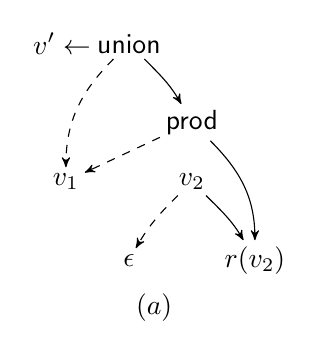
\begin{tikzpicture}[->,>=stealth',roundnode/.style={circle,draw,inner sep=1.2pt},squarednode/.style={rectangle,inner sep=2pt}, scale=1]
		\node [squarednode] (c) at (1.12, -0.6) {$(a)$};
		\node [squarednode] (0) at (0.8, 2.75) {$\textsf{union}$};
		\node [squarednode] (6) at (-0.05, 2.75) {$v'\gets$};
		\node [squarednode] (1) at (0, 1) {$v_1$};
		\node [squarednode] (2) at (1.6, 1.75) {$\textsf{prod}$};
		\node [squarednode] (3) at (1.6, 1) {$v_2$};
		\node [squarednode] (4) at (0.8, 0) {$\epsilon$};
		\node [squarednode] (5) at (2.4, 0) {$r(v_2)$};
		\draw[dashed] (0) to[out=-135,in=90] (1);
		\draw (0) to[out=-45,in=120] (2);
		\draw (2) to[out=-45,in=90] (5);
		\draw[dashed] (3) to[out=-135,in=60] (4);
		\draw (3) to[out=-45,in=120] (5);
		\draw[dashed] (2) to (1);
	\end{tikzpicture}
	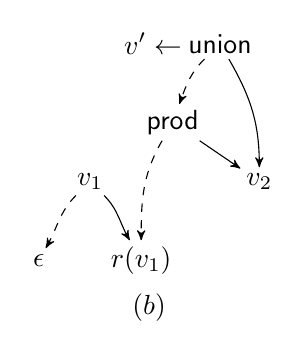
\begin{tikzpicture}[->,>=stealth',roundnode/.style={circle,draw,inner sep=1.2pt},squarednode/.style={rectangle,inner sep=2pt}, scale=1]
		\node [squarednode] (c) at (1.6, -0.6) {$(b)$};
		\node [squarednode] (0) at (2.5, 2.75) {$\textsf{union}$};
		\node [squarednode] (6) at (1.65, 2.75) {$v'\gets$};
		\node [squarednode] (1) at (3, 1) {$v_2$};
		\node [squarednode] (2) at (1.90, 1.75) {$\textsf{prod}$};
		\node [squarednode] (3) at (0.85, 1) {$v_1$};
		\node [squarednode] (4) at (0.2, 0) {$\epsilon$};
		\node [squarednode] (5) at (1.5, 0) {$r(v_1)$};
		\draw (0) to[out=-60,in=90] (1);
		\draw[dashed] (0) to[out=-135,in=70] (2);
		\draw[dashed] (2) to[out=-120,in=90] (5);
		\draw[dashed] (3) to[out=-135,in=60] (4);
		\draw (3) to[out=-45,in=120] (5);
		\draw (2) to (1);
	\end{tikzpicture}
	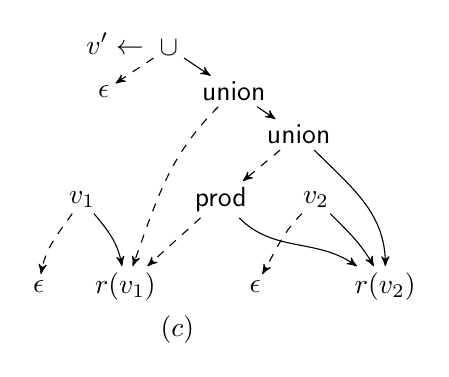
\begin{tikzpicture}[->,>=stealth',roundnode/.style={circle,draw,inner sep=1.1pt},squarednode/.style={rectangle,inner sep=2pt},scale=1.1]
		\node [squarednode] (c) at (1.6, -0.5) {$(c)$};
		\node [squarednode] (0) at (1.5, 2.75) {$\cup$};
		\node [squarednode] (11) at (0.88, 2.8) {$v'\gets$};
		\node [squarednode] (1) at (0.75, 2.25) {$\epsilon$};
		\node [squarednode] (2) at (2.25, 2.25) {$\textsf{union}$};
		\node [squarednode] (3) at (3, 1.75) {$\textsf{union}$};
		\node [squarednode] (4) at (2.1, 1) {$\textsf{prod}$};
		\node [squarednode] (5) at (3.2, 1) {$v_2$};
		\node [squarednode] (6) at (2.5, 0) {$\epsilon$};
		\node [squarednode] (7) at (4, 0) {$r(v_2)$};
		\node [squarednode] (8) at (0.5, 1) {$v_1$};
		\node [squarednode] (9) at (0, 0) {$\epsilon$};
		\node [squarednode] (10) at (1, 0) {$r(v_1)$};
		\draw[dashed] (0) to (1);
		\draw (0) to (2);
		\draw[dashed] (2) to[out=-135,in=70] (10);
		\draw[dashed] (4) to (10);
		\draw (4) to[out=-45,in=145] (7);
		\draw[dashed] (5) to[out=-135,in=60] (6);
		\draw (5) to[out=-45,in=120] (7);
		\draw (3) to[out=-45,in=90] (7);
		\draw[dashed] (3) to (4);
		\draw (2) to (3);
		\draw (8) to[out=-50,in=100] (10);
		\draw[dashed] (8) to[out=-125,in=80] (9);
	\end{tikzpicture}
	\caption{Gadgets for product as defined for an $\cD$ with the $\epsilon$-node.}
	\label{fig:prod-multi-gadget}
\end{figure}

Lorem ipsum dolor sit amet, consectetur adipiscing elit, sed do eiusmod tempor incididunt ut labore et dolore magna aliqua. Ut enim ad minim veniam, quis nostrud exercitation ullamco laboris nisi ut aliquip ex ea commodo consequat. Duis aute irure dolor in reprehenderit in voluptate velit esse cillum dolore eu fugiat nulla pariatur. Excepteur sint occaecat cupidatat non proident, sunt in culpa qui officia deserunt mollit anim id est laborum.

	
\end{document}
